\chapter{Literature}
    In this chapter, some basic knowledge of deep learning neural network for vision tasks, i.e. keypoints detection, will be introduced at the beginning. 
    More specifically, Some works about Wire harness detection using AI method will be presented. Additionally, some state of the art methods and architectures, 
    which might improve the precision of keypoints detection of wire harnessed will also be presented. After that, some approaches for generating datasets 
    artificially and expanding datasets are introduced at the end.
\section{Deep neural network for vision tasks}
    Recently, using deep neural network for vision tasks becomes a popular choice for researchers, for example, Image Classification\cite{8016501}, 
    Object detection\cite{10028728}, Human pose estimation\cite{Sun_2019_CVPR}, Semantic Segmentation\cite{HAO2020302}. Compare with the some 
    tradition computer vision technologies, the approach provide more satisfactory results\cite{voulodimos2018deep}. 
    In this section, some of the most important deep learning network structures for vision tasks will be introduced. Object and keypoints
    detection will be the highlights due to their close connection with the tasks of the thesis.\\
\textbf{Object detection}\\
    The goals of object detection are: what(classification) and where(locolization) is the object is. \autoref{fig:object detection} is an example of object
    detection. In this image, the branches of wire harness is bounded by a green box as groundtruth. They are classified as branches and the locations could 
    also be detected. It serves as the basic of some deep learning based computer vision task such as instance segmentation and object tracking\cite{10028728}. 
    \begin{figure}
        \centering
        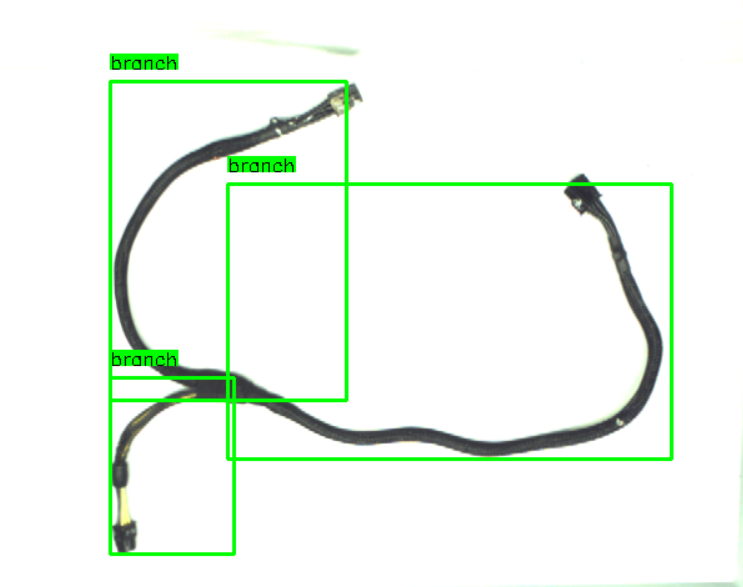
\includegraphics[width=0.6\linewidth]{example_images/object detection}
        \caption{Ground truth of Object detection}
        \label{fig:object detection}
    \end{figure}
    In \cite{Girshick_2014_CVPR}, the authors present a method called R-CNN(Region-based Convolutional Network), which improves the accuracy of object detection. 
    The approach consists of three modules:
    \begin{itemize}
        \item [(1)] \textbf{Region proposals: }In this module, category-independent region proposals will be generated.
        \item [(2)] \textbf{Feature extractions: }The features will be extracted using CNN \cite{NIPS2012_c399862d}.
        \item [(3)] \textbf{Classification: }At last the classification task is done by a set of classspecific linear SVMs. 
    \end{itemize}
    After one years, Ross Girshick proposed an optimized method named Fast R-CNN in 2015\cite{Girshick_2015_ICCV}. Compared with all objects on image are passed 
    through the neural network in R-CNN,  in Fast R-CNN the whole images will be passed forward together to extract the features, which improves the efficiency 
    significantly. Faster R-CNN combined Fast R-CNN with Region Proposal Networks(RPN), which outputs a set of rectangular object proposals, each with an objectness
    score\cite{NIPS2015_14bfa6bb}. It is trained end-to-end to generate high-quality region proposals, which are passed to Fast R-CNN for object detection tasks.
    This method simplified the process further and the model is easier to be trained.\\
    The above introduced models are from R-CNN family. Joseph Redmon proposed a new model named YOLO, whose pipeline has just one simple network. It could also be 
    trained end-to-end extremely fast\cite{Redmon_2016_CVPR}. The detection task will be framed as a regression problem to spatially separated bounding boxes and
    associated class probabilities. Due to the rapidity, it is widely used in the task of real-time object detection. After an eight-year development, the Tsinghua 
    University team presented the tenth generation of the YOLO model in 2024\cite{wang2024yolov10}. Today, the YOLO model integrates state-of-the-art deep learning 
    techniques, such as an enhanced version of CSPNet\cite{Wang2019CSPNetAN} as the backbone network, PAN (Path Aggregation Network) for effective multi-scale feature
    fusion\cite{Liu_2018_CVPR}. This enables fast and accurate real-time object detection.
    Kaiming HE from Facebook AI Research extended Faster R-CNN\cite{NIPS2015_14bfa6bb} and prensented 
